%!TEX TS-program = xelatex
%!TEX encoding = UTF-8 Unicode
%!TeX spellcheck = it_IT
%!TEX root = ../tesi.tex

\chapter{Simulazioni}\label{chap:simulazioni}
% INTRO: cosa c'è in questa sezione?
Dopo aver illustrato il protocollo in esame e il modello di propagazione utilizzato si passa ora alla fase di valutazione.
Il capitolo procederà nel dettaglio dei diversi scenari affrontati,
illustrandone le motivazioni e le caratteristiche e discutendo i risultati ottenuti.
%
\section{Scenario a griglia}\label{sec:configurazione-griglia}
% \subsection{Panoramica}
% Simulazioni codice barichello:
%  - struttura simulazioni
%  - grafici
%  - risulati
Il primo gruppo di simulazioni ha lo scopo di analizzare l'impatto degli edifici sul comportamento del protocollo
Fast Broadcast all'interno di uno scenario conosciuto, ossia quello presentato nella tesi originale~\cite{Barichello2017propagazione}
a cui sono stati aggiunti degli edifici.
La configurazione dello scenario, dei nodi e della rete è la stessa ed è riassunta in Tabella~\ref{tab:parametri-simulazioni-barichello}.
L'ambiente è una città fittizia con strade a griglia in stile Manhattan di lunghezza $4000$ metri e distanti l'una dall'altra $300$ metri.
I veicoli sono disposti a $12$ metri di distanza per un totale di $8064$.
Il veicolo che da inizio alla fase di inoltro (generazione del primo messaggio di inoltro),
che per facilità verrà chiamato veicolo \textit{zero}, è posizionato al centro della griglia.
Seguendo l'idea originale, è stata definita anche un circonferenza di raggio pari a $1000\pm12$ metri utilizzata per definire alcune metriche di valutazione;
la circonferenza ha centro in corrispondenza del veicolo zero.
Il raggio trasmissivo effettivo (fisico) assume due valori possibili: $300$ o $500$ metri.
%
\begin{table}[!h]
	\centering
	\begin{tabular}{| L{.4\linewidth} | r  l |}
		\toprule
		Parametro															&			Valore 							&					\\
		\thickerline
		Lunghezza delle strade								&			$4000$							& m				\\
		Distanza fra le strade								&			$300$								& m				\\
		Distanza fra i veicoloi								&			$12$ 								& m				\\
		Circonferenza													&			$1000\pm12$					& m				\\
		Posizione del veicolo zero						&			centrale						&					\\
		\thickerline
		Dimensioni pacchetto									&				$164$							&			byte		\\	\hline
		Standard trasmissione									&				$802.11$b					&							\\	\hline
		Frequenza															&				$2.4$							&			GHz			\\	\hline
		Banda del canale											&				$22$							&			MHz			\\	\hline
		Velocità di trasmissione							&				$11$							&			Mbps		\\	\hline
		Potenza trasmissione									&				$7,5$							&			dBm			\\	\hline
		Raggio trasmissivo										&				$300$-$500$				&			m				\\	\hline
		Codifica															&				DSSS\footnotemark	&							\\	\hline
		Modello di propagazione								&				\textsf{ns3::RangePropagation}	&							\\	\hline
		Modello di ombreggiatura							&				A ostacoli				&							\\	\hline
		\thickerline
		Simulazioni	per configurazione				&			$50$								&					\\
		\bottomrule
	\end{tabular}
	\caption{Configurazione dei parametri per le simulazioni.\label{tab:parametri-simulazioni-barichello}}
\end{table}
\footnotetext{\textit{Direct Sequence Spread Spectrum}}	% TODO controllare la posizone, che sia nella stessa pagina della tabella.
%
Per valutare il protocollo sono stati presi in esame diversi parametri: la copertura totale e la copertura sulla circonferenza,
il numero di salti necessari a raggiungere il bordo della griglia, il numero totale di messaggi di inoltro ricevuti e inviati.
Per poter confrontare le prestazioni del protocollo Fast Broadcast, quest'ultimo è stato comparato con altri due metodi chiamati \statica e \staticb,
che utilizzano una stima fissa del raggio tramissivo rispettivamente di $300$ e $500$ metri.
Il raggio trasmissivo varia agendo sul modello di propagazione \textsf{ns3::RangePropagation},
implementazione di ns-3 del modello a disco unitario, nel quale una trasmissione viene ricevuta se è a una distanza minore o uguale della portata impostata.
Gli edifici, non presenti nello scenario originale, sono stati creati manualmente in modo che ogni edificio fosse contenuto all'interno dello spazio creato dalle strade.
Così facendo, risultano $169$ edifici di $295$x$295$ metri (i muri sono distanziati di $5$ metri dalla strada).

Le simulazioni sono state eseguite sfruttando l'attrezzatura in dotazione al servizio di \textit{High Performance Computing} dell'università di Padova,
% mettere anche il tempo?
eseguendono un numero pari a $50$ simulazioni per ogni configurazione.
%
% \begin{figure}[htbp]
% 	\centering
% 	\begin{center}
% 		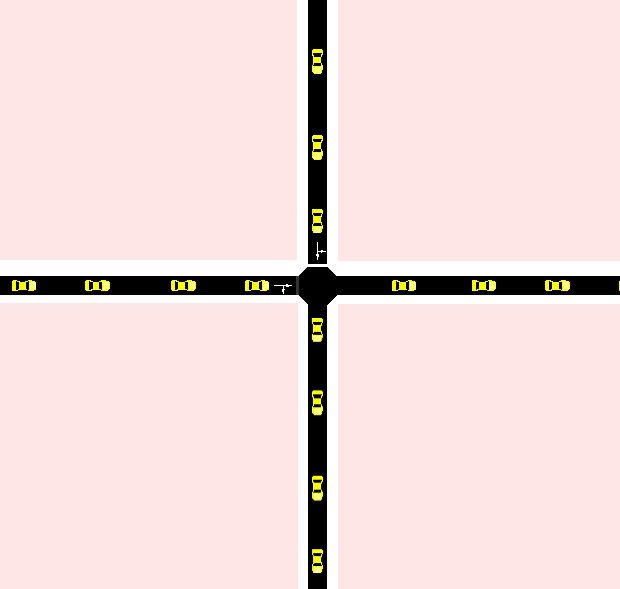
\includegraphics[width=.4\textwidth]{griglia-dettaglio-2.png}
% 	\end{center}
% 	\label{fig:griglia-dettaglio}\caption{Dettaglio della configurazione a griglia: in nero le strade e in giallo gli edifici.}
% \end{figure}
%
\subsection{Risultati}\label{sec:configurazione-griglia-risultati}
I grafici dalla \figurename~\ref{fig:risultati-griglia-copertura} alla~\ref{fig:risultati-griglia-messaggi}\footnotemark
\footnotetext{Tutti i grafici mostrati utilizzano come misura di errore l'errore standard con intervallo di confidenza del $95\%$.}
mostrano i risultati di questo gruppo di simulazioni.
Come si può notare, la presenza degli ostacoli influisce molto poco sui quasi tutti i parametri presi in esame.
La differenza sulla copertura totale è, in generale, inferiore o vicina all'$1\%$, tuttavia utilizando i protocolli FB e \statica{} si vede
un leggero calo nel caso di raggio tramissivo pari a $300$m e un leggero incremento con $500$m, mentre
è l'opposto con \staticb{}; la differenza è comunque minima per ipotizzare la causa di questo comportamento. % ?
I veicoli sulla circonferenza (di raggio $1000$m) ottengono una copertura legggermente migliore
(in media dello $0,5\%$), tranne nel caso di \staticb{} con raggio trasmissivo $500$m.
Questo leggero aumento della copertura potrebbe essere dovuto a quello che gli autori del modello a ostacoli (~\cite{Carpenter:2015:OMI:2756509.2756512})
chiamano ``L'effetto cena con amici'' (\textit{The Dinner Party effect}): la presenza di ostacoli come edifici
può aumentare, localmente, la probabilità di tramissioni con successo in quanto aumenterebbe il riuso delle spazio.
Tale fenomeno può anche essere visto nel grafico in \figurename~\ref{fig:risultati-griglia-messaggi}
dove nel caso di raggio trasmissivo pari a $500$m è presente un aumento, in media, del $5,6$\%
nel numero di messaggi di inoltro ricevuti, mentre quelli inviati sono più simili al caso senza edifici.
Anche il numero di salti necessari a raggiungere il perimetro della griglia rimane vicino
e aumenta mediamente solo del $0,34\%$.
Da tutto ciò si deduce che la presenza di edifici causa un aumento locale del traffico di messaggi
ma il meccanimo di contesa e inoltro permette di mantenere limitata la propagazione di questi in avanti. % sicuro?
Ciascun edificio ricopre un intero isolato (spazio interno racchiuso fra le strade) e si trova, per una differenza di pochi metri,
a ridosso delle strade;
la grandezza di questi edifici probabilmente blocca qualsiasi trasmissione fra due veicoli che si trovano
agli estremi dell'isolato e, di conseguenza, limita la propagazione del messaggio all'interno del blocco  che viene ``forzato''
a proseguire lungo la strada.
%
\begin{figure}[htbp]
	\centering
		\includegraphics[width=\linewidth]{grafici/griglia/copertura_totale.png}
		\includegraphics[width=\linewidth]{grafici/griglia/copertura_circonferenza.png}
\caption{Scenario a griglia: copertura dei veicoli in totale e sulla circonferenza.\label{fig:risultati-griglia-copertura}}
\end{figure}
%
\begin{figure}[htbp]
	\centering
		\includegraphics[width=\linewidth]{grafici/griglia/salti.png}
\caption{Scenario a griglia: numero di salti.\label{fig:risultati-griglia-salti}}
\end{figure}
%
\begin{figure}[htbp]
	\centering
		\includegraphics[width=\linewidth]{grafici/griglia/messaggi_inviati.png}
		\includegraphics[width=\linewidth]{grafici/griglia/messaggi_ricevuti.png}
\caption{Scenario a griglia: numero di messaggi di inoltro inviati e ricevuti.\label{fig:risultati-griglia-messaggi}}
\end{figure}
\clearpage
%
%
\section{Scenario urbano reale}\label{sec:configurazione-la-pd} % un titolo migliore no?
Le configurazioni precedenti avevano il difetto di essere poco veritiere, dal punto di vista della topologia stradale
che sulla geometria degli edifici.
Le strade formavano una griglia perfetta, con strade identiche e incroci esatti;
gli edifici erano molto grandi e tutti della stessa forma e dimensione.
In questo gruppo di simulazioni, invece, si è cercato di rappresentare un vero scenario realistico,
con strade di lunghezza diversa e non perfettamente allineate,
con edifici meno squadrati, a ridosso della strada o anche assenti in alcune zone (difficile in città, ma possibile).

A questo proposito sono state scelte due città, Padova (IT) e Los Angeles (California, USA) (Figura~\ref{fig:scenari-la-pd-osm}), definite due aree nella zona centrale di circa $5$ kilometri quadrati
e, seguendo il procedimento descritto nella Sezione~\ref{sec:sumo}, sono state estratte le informazioni necessarie alla configurazione delle simulazioni.
Altre informazioni sugli scenari e sui parametri delle rete (se diverse dalle precedenti) sono elencati in Tabella~\ref{tab:parametri-simulazioni-pd-la}.
La scelta è ricaduta su Los Angeles poiché la sua rete stradale è paragonabile a una griglia in stile Manhattan, come nello scenario precedente,
mentre Padova (sede anche dell'Università dove si è svolto questo lavoro) ha una toplogià più irregolare, con strade più strette ed edifici a ridosso di queste,
zone pedonali e ZTL.
In questo modo si ha uno scenario che si avvicina al precente come concezione,
una sua versione reale, mentre un secondo con caratteristiche proprie.

In questo gruppo di simulazioni sono state utilizzate le medesime metriche del caso precendente,
fatta eccezione per il numero di salti che ora sono per raggiungere la circonferenza, invece che il perimetro della mappa.
Questo perché nella configurazione a griglia lungo il bordo esterno erano sicuramente posizionati dei veicoli,
mentre ora il limite ``quadratico'' dell'area è ideale.

Inoltre, per rappresentare al meglio il mezzo trasmissivo è stato utilizzato come modello di propagazione base
quello a doppio raggio (Two-Ray Ground), in quanto quello precedente (portata fissa) non teneva in considerazione
diversi parametri essenziali, come la potenza della trasmissione, la frequenza del segnale o l'altezza delle antenne rispetto al suolo;
inoltre l'assunzione che il segnale si propaghi uniformemente fino a una certa distanza prefissata è poco reale.
%
\begin{table}[htbp]
	\centering
	  \begin{tabular}{| L{.35\linewidth} | C{.01\linewidth} | C{.04\linewidth} | L{.15\linewidth} | L{.15\linewidth} |}
			\toprule
			\multicolumn{3}{|m{.3\linewidth}|}{\multirow{2}{*}{}}														&		\multicolumn{2}{c|}{Scenario}						\\ \cline{4-5}
			\multicolumn{3}{|m{.3\linewidth}|}{}																						&		Padova				&			Los Angeles					\\
			\thickerline
			\multicolumn{2}{|m{.25\linewidth}|}{\multirow{2}{*}{Latitudine}}				&		N	 	& 	$45,4171$				&			$33,9654$					\\ \cline{3-5}
			\multicolumn{2}{|m{.25\linewidth}|}{}																		&		S	 	& 	$45,3981$				&			$33,9478$					\\ \hline
			\multicolumn{2}{|l|}{\multirow{2}{*}{Longitudine}}											&		O	 	& 	$11,8654$				&			-$118,3260$				\\ \cline{3-5}
			\multicolumn{2}{|l|}{}																									&		E	 	& 	$11,8923$				&			-$118,3055$				\\ \hline
			\multicolumn{3}{|l|}{Area approssimativa [km$^2$]}															&		\multicolumn{2}{c|}{$5$}								\\ \hline
			\multicolumn{3}{|l|}{Distanza fra veicoli [metri]}															&		\multicolumn{2}{c|}{$25$}								\\ \hline
			\multicolumn{3}{|l|}{Numero di veicoli}																					&		$2224$					&					$1905$				\\ \hline
			\multicolumn{3}{|l|}{Numero di ostacoli}																				&		$6322$					&					$8241$				\\ \hline
			\multicolumn{3}{|l|}{Potenza trasmissione [dBm]}																	&		\multicolumn{2}{c|}{$4,6$-$13,4$}						\\	\hline
			\multicolumn{3}{|l|}{Modello di propagazione}																		&		\multicolumn{2}{c|}{\textsf{ns3::TwoRayGround}}		\\	\hline
			\thickerline
			\multicolumn{3}{|l|}{Simulazioni	per configurazione}														&		\multicolumn{2}{c|}{$50$}					\\
			\bottomrule
	  \end{tabular}
	\caption{Parametri della topologia per gli scenari urbani.\label{tab:parametri-simulazioni-pd-la}}
\end{table}
%
\begin{figure}[htbp]
	\centering
		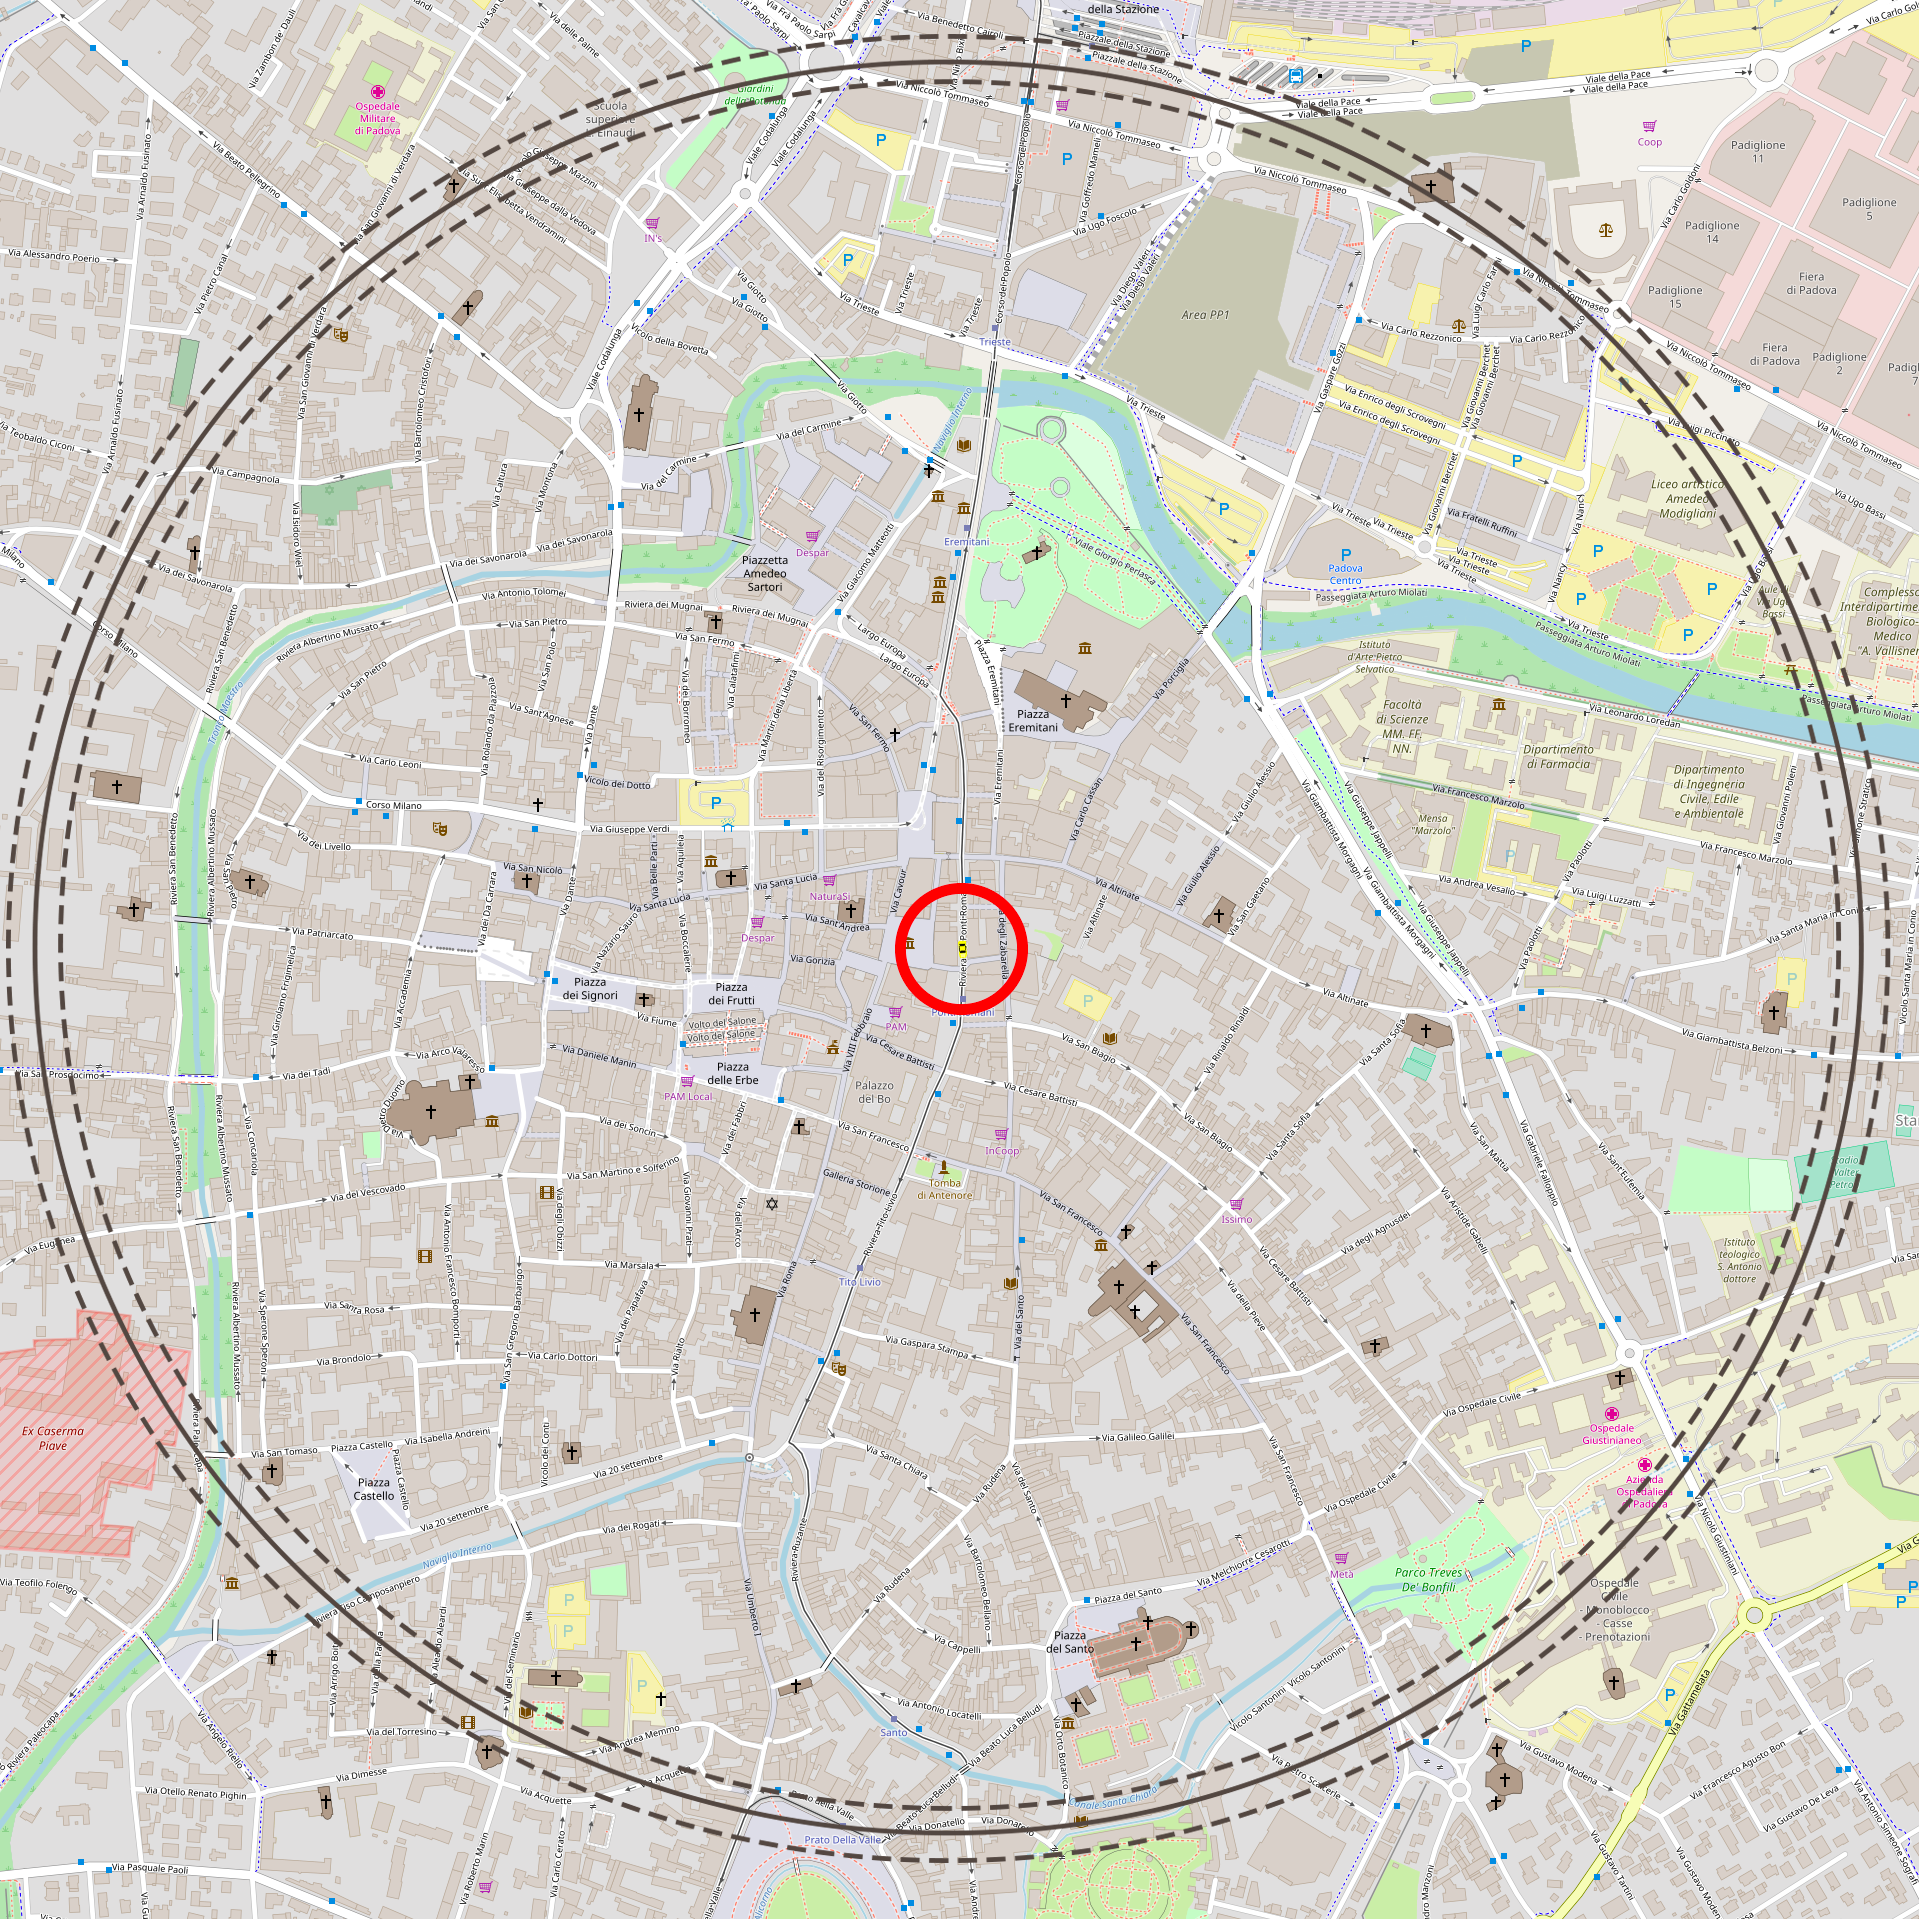
\includegraphics[width=.65\textwidth]{osm_web-pd-2x2.png}
		\vspace{10pt}
		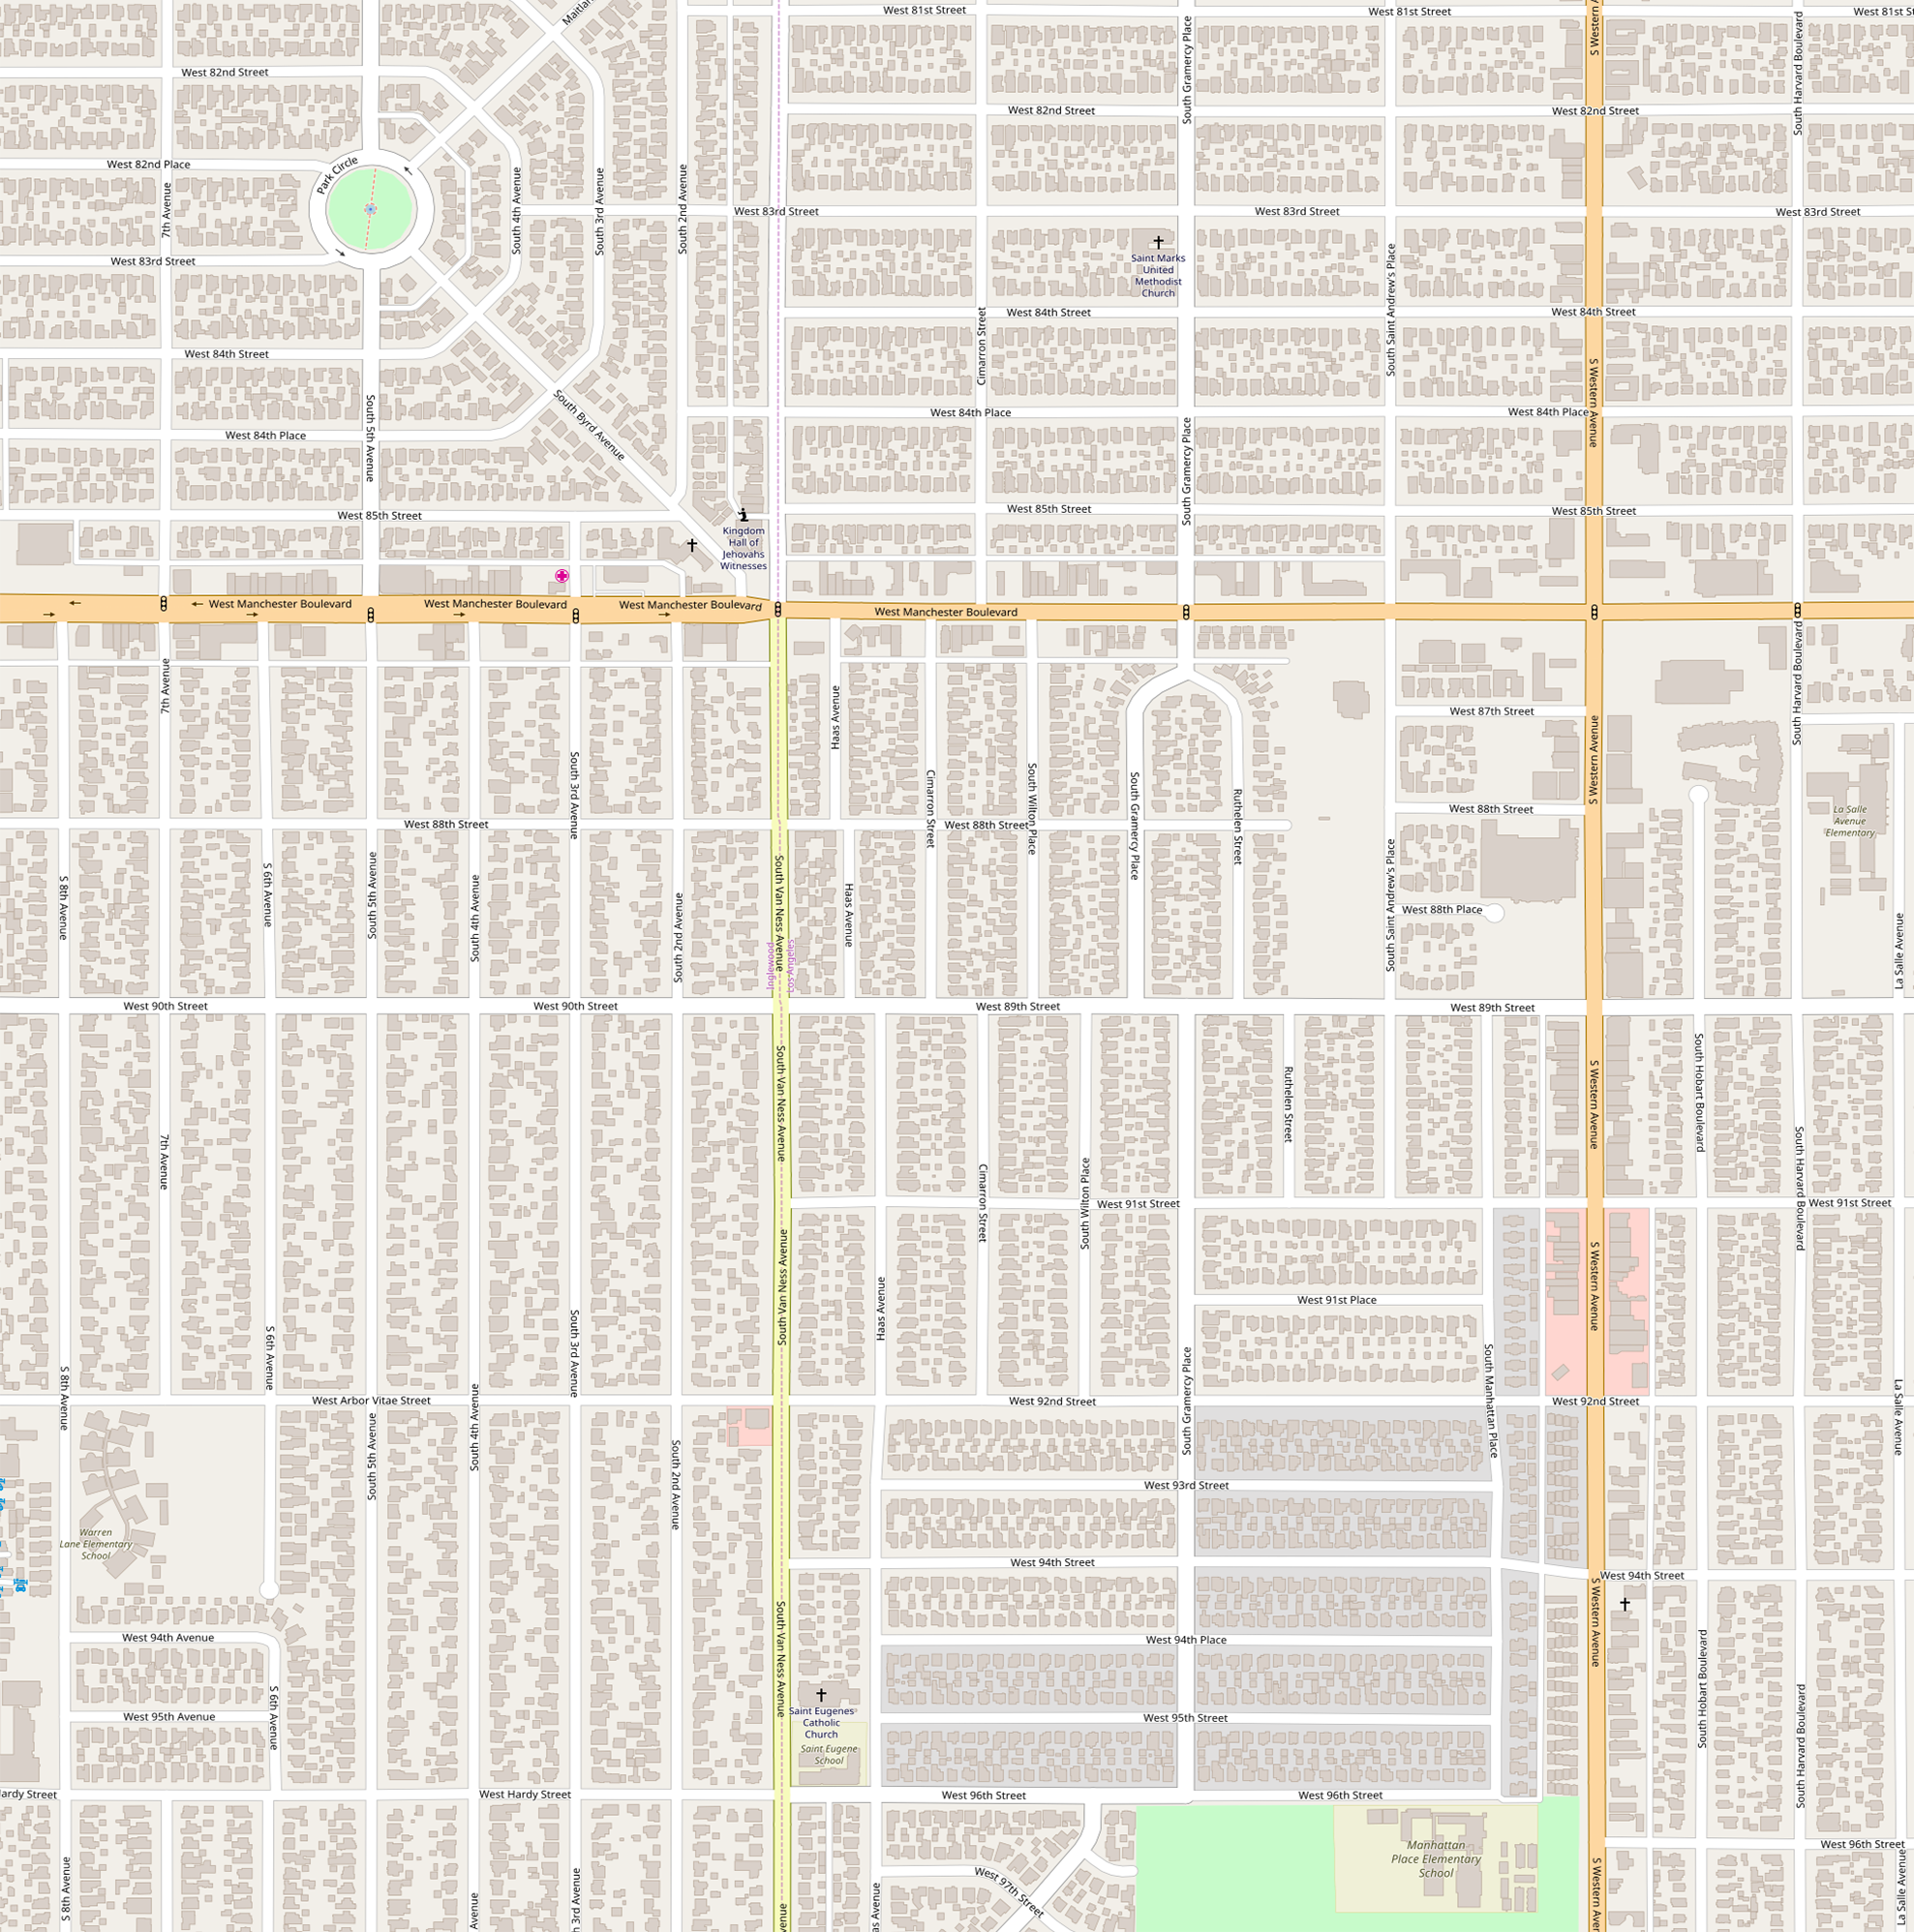
\includegraphics[width=.65\textwidth]{osm_web-la-2x2.png}
\caption{Una vista delle aree selezionate per le simulazioni; a sinistra la città di Padova e a destra Los Angeles (fonte: OSM).
Il cerchio rosso evidenzia la posizione del nodo di partenza mentre i tre rimanenti rappresentano il perimetro della circonferenza
e i due intervalli di confidenza.\label{fig:scenari-la-pd-osm}}
\end{figure}
%
\subsection{Los Angeles}\label{subsec:risultati-la}
A differenza del precente, quando si va a considerare l'effetto dell'ombreggiatura in questo scenario
si notano dei maggiori cambiamenti.
In primo luogo, come si può vedere dalla \figurename~\ref{fig:risultati-la-copertura},
è presente una diminuzione della copertura dei veicoli che è più marcata con raggio trasmissivo $300$m.
Nelle simulazioni, infatti, le due diverse distanze massime raggiungibili dal segnale,
$300$ e $500$ metri senza ostruzioni, sono state implementate tramite una diversa potenza in fase di trasmissione.
Un sengale più potente ha, naturalmente,
più probabilità di ``superare'' un ostacolo rispetto a un segnale con meno potenza.
Inoltre, avendo una portata maggiore potrebbe raggiungere altri elementi in ricezione,
permettere degli inoltri e coprire ulteriori veicoli.
Da notare è il cambio di tendenza nel caso del protocollo \statica{}:
in presenza di edifici si ha una copertura maggiore con raggio trasmissivo di $500$m.
Il motivo potrebbe essere che l'effetto dell'ombreggiatura influisce maggiormente rispetto
allo non stimare correttamente il mezzo fisico.
Questo fenomeno rimarrà costante anche nello scenario successivo.

Per quanto riguarda il numero medio di salti necessari a raggiungere i veicoli sulla circonferenza,
in \figurename~\ref{fig:risultati-la-salti},
% TODO: contorllare che sia così anceh avendo nuovi dati
si ha un incremento del $36,5\%$ nel caso di raggio trasmissivo $300$m mentre solo del $5\%$ nella controparte a $500$m.
Inoltre, si può osservare come il protocollo FB abbia prestazioni migliori delle alternative statiche
di circa il $10\%$ con $300$m e del $23\%$ con $500$m. % ha senso confrontarli così?
Considerando il numero di messaggi di inoltro che vengono scambiati nella rete (\figurename~\ref{fig:risultati-la-messaggi}),
rimane anomalo il caso \statica{}-$500$m, dove si ha un valore inferiore rispetto agli altri protocolli,
anche se rimane coerente nel considerare l'effetto ombreggiatura (rispetto allo scenario senza).
Mediamente, i messaggi inviati nel caso $300$m subiscono un incremento del $194,5\%$ e del $179,4\%$
con $500$m.
Un andamento inverso caratterizza il numero totale di messaggi di inoltro ricevuti:
se si considera un raggio trasmissivo di $500$m si ha un aumento del $43\%$ in presenza di edifici,
mentre un calo del $32,2\%$ con $300$m.
Ciò significa che nel primo caso gli ostacoli considerati causano la perdita di una grossa quantità di messaggi
mentre così non avviene nel secondo.
La causa di questo fenomeno potrebbe trovarsi nella topologia stradale presente in questo specifico scenario:
gli isolati più piccoli hanno una dimensione di circa $50$x$175$ metri mentre quelli più grandi
(visibili nella mappa in basso a destra) sono lunghi circa $400$ metri.
Il raggio trasmissivo minore non riesce a superarli mentre è così per quello maggiore che raggiunge
di conseguenza anche i veicoli posizionati sugli e nelle vicinanze degli incroci.
Considerando gli isolati più piccoli con $300$m si coprono (al massimo) due incroci mentre se ne coprono
fino a tre se si hanno $500$m.
Inoltre, potrebbe essere che il segnale generato nel caso di raggio trasmissivo minore
non sia sufficiente a penetrare gli edifici presenti all'interno di un isolato (in larghezza),
mentre è abbastanza forte quello con raggio trasmissivo maggiore.

Osservando i grafici si nota una maggior variabilità dei dati quando si considerano gli ostacoli.
Questo può voler dire che per avere risultati più stabili è necessario eseguire più simulazioni
con ostacoli rispetto alla controparte che non li considera.
Questo fenomeno è più visibile con il protocollo FB che a differenza degli altri
ha una componente probabilistica in più, ossia lo scambio iniziale di messaggi Hello.
Ciò potrebbe voler dire anche che per effettuare una buona stima del raggio trasmissivo
sono necessari più scambi di messaggi di quelli che si erano visti non considerando gli ostacoli. % --> sicuro? boh

Anche in questo scenario, il protocollo FB si comporta secondo le aspettative
garantendo una copertura migliore % TODO da confermare dopo con i nuovi dati
rispetto ai protocolli con stima fissa,
un numero di salti inferiore e quindi una consegna del messaggio più veloce
e in generale un numero inferiore di messaggi inoltrati.
%
\begin{figure}[htbp]
	\centering
		\includegraphics[width=\linewidth]{grafici/la/copertura_totale.png}
		\includegraphics[width=\linewidth]{grafici/la/copertura_circonferenza.png}
\caption{Scenario L.A.: copertura dei veicoli in totale e sulla circonferenza.\label{fig:risultati-la-copertura}}
\end{figure}
%
\begin{figure}[htbp]
	\centering
		\includegraphics[width=\linewidth]{grafici/la/salti.png}
\caption{Scenario L.A.: numero di salti.\label{fig:risultati-la-salti}}
\end{figure}
%
\begin{figure}[htbp]
	\centering
		\includegraphics[width=\linewidth]{grafici/la/messaggi_inviati.png}
		\includegraphics[width=\linewidth]{grafici/la/messaggi_ricevuti.png}
\caption{Scenario L.A.: numero di messaggi di inoltro inviati e ricevuti.\label{fig:risultati-la-messaggi}}
\end{figure}
\clearpage
%
%
\subsection{Padova}\label{subsec:risultati-pd}
% TODO: rivedere tutti qiesti risultati
Similmente ai risultati ottenuti nelle simulazioni precendenti,
anche nel centro cittadino padovano si subisce una brusca riduzione della copertura totale
quando si va a considerare l'effetto ombreggiatura casuato dagli edifici (\figurename~\ref{fig:risultati-padova-copertura}).
Più precisamente, in questo caso il calo è maggiore e pari al $49,5\%$ nel caso $300$m,
a differenza del precente che si attestava al $30,5\%$;
utilizzando il raggio trasmissivo pari a $500$m la differenza di copertura totale si attesta
intorno al $9\%$ per entrambi gli scenari.
Una sostanziale differenza di nota anche nella copertura dei veicoli che si trovano sulla circonferenza,
dove si registra un calo che arriva fino al $77,3\%$ con \statica{}-$300$m;
lungo questo raggio si trovano $50$ veicoli ma nel caso $300$m se ne copre mediamente solo il $24,5\%$.
Se ne deduce che alcune caratteristiche intrinseche della città veneta
impattano maggiormente un raggio trasmissivo minore che uno maggiore rispetto
alle equivalenti della città californiana. % è giusto scriver così?
Questo potrebbe essere dovuto alla geometria e topologia degli edifici della città
veneta, a ridosso della careggiata, più stipati e con meno spazio libero,
oppure dalla diverse struttura stradale, che vede strade più strette,
rettilinei di lunghezza inferiore e cambi di direzione repentini.

Per quanto riguarda il numero di salti (per raggiungere la circonferenza) in \figurename~\ref{fig:risultati-padova-salti},
i risultati sono coerenti con le aspettative e con lo scenario Los Angeles:
il protocollo Fast Broadcast si comporta leggermente peggio in Padova che in L.A.
ma rimane il migliore nell'adattarsi al cambiamento di raggio trasmissivo reale.

Rimane l'anomalia nel caso \statica{}-$500$m del numero di messaggi di inoltro in \figurename~\ref{fig:risultati-padova-messaggi},
dove si ha un valore inferiore rispetto al protocollo statico con stima corretta.
Come nello scenario precedente, la causa potrebbe essere la maggior influenza dell'ombreggiatura rispetto
all'effettuare una stima corretta del mezzo fisico.
Considerando l'effetto degli edifici si ha un aumento dei messaggi inviati del $234\%$ nel caso $300$m e del $197\%$ nell'altro,
un incremento maggiore rispetto allo scenario precente probabilmente per le stesse cause
descritte in precedenza osservando gli effetti sulla copertura dei veicoli.
Nel numero di messaggi di inoltro ricevuti si ha un calo nel caso $300$m,
pari al $44,9\%$, e un aumento con il raggio trasmissivo maggiore, del $46,9\%$,
come nelle simulazioni con la città californiana.
%
\begin{figure}[htbp]
	\centering
		\includegraphics[width=\textwidth]{grafici/pd/copertura_totale.png}
		\includegraphics[width=\textwidth]{grafici/pd/copertura_circonferenza.png}
\caption{Scenario Padova: copertura dei veicoli in totale e sulla circonferenza.\label{fig:risultati-padova-copertura}}
\end{figure}
%
\begin{figure}[htbp]
	\centering
		\includegraphics[width=\textwidth]{grafici/pd/salti.png}
\caption{Scenario Padova: numero di salti.\label{fig:risultati-padova-salti}}
\end{figure}
%
\begin{figure}[htbp]
	\centering
		\includegraphics[width=\textwidth]{grafici/pd/messaggi_inviati.png}
		\includegraphics[width=\textwidth]{grafici/pd/messaggi_ricevuti.png}
\caption{Scenario Padova: numero di messaggi di inoltro inviati e ricevuti.\label{fig:risultati-padova-messaggi}}
\end{figure}
\clearpage
%
%
\section{Scenario urbano con sensori}\label{sec:configurazione-sensori}
Inizialmente si era detto che spesso le reti VANET sono caratterizzate da nodi con capacità di comunicazione
intra-veicolare e che, grazie ai progressi tecnologici, sempre più veicoli possiedono queste caratteristiche.
Tuttavia bisogna prendere atto che, almeno per il momento, non siamo nelle condizioni
di poter affermare che ogni ogni veicolo è grado di comunicare.
Per questo motivo, si può pensare di rilassare tale assunzione e permettere che alcuni veicoli
siano esclusi dal traffico; la loro presenza all'interno dello scenario rimane ma non partecipano allo scambio di messaggi.

Viene aggiunta una seconda assunzione: sparpagliati lungo la città sono posizionati dei sensori a basso costo
che contribuiscono alla propagazione dei messaggi tramite il semplice Algortimo~\ref{fig:algoritmo-inoltro-dummy}
che inoltra (in broadcast) un messaggio solo la prima volta.
%
\begin{italianalgorithm}[h]
\begin{algorithmic}[1]
	\If{(RilevatoMsg() $\wedge$ visto() = NO)}
		\State{visto $\gets$ SI}
		\State{inviaInBroadcast(msg)}
		\EndIf{}
\end{algorithmic}
\caption{Semplice algoritmo di inoltro.}\label{fig:algoritmo-inoltro-dummy}
\end{italianalgorithm}
%
Nel mondo reale questi sensori potrebbero essere dedicati come aiuto propagazione,
cioè installati al solo scopo di aiutare la diffusione dei messaggi
oppure essere presenti per altri motivi ma con la capacità di ricevere/inoltrare messaggi
in caso di bisogno; ad esempio sensori per l'analisi delle polveri sottili,
oppure per il monitoraggio del traffico stradale.
Si assume, inoltre, che questi sensori siano posizionati a una certa altezza prefissata;
potrebbe essere che, in fase di installazione si sia scelto di utilizzare delle infrastrutture
pre-esistenti, come per esempio delle lanterne semaforiche, sulle quali montare i sensori in modo da ridurre i costi.
Prendendo come spunto l'esempio indicato, si è visto che nel classico semaforo a tre tempi
la parte contenente i segnali luminosi dev'essere posizionata
fra i $15$ e i $26,5$ piedi (rispettivamente $4,5$ e ho $8$ metri) nel caso di strutture al di sopra della
careggiata~\cite{MUTCD}.

Nel dettaglio, lo scenario attuale prevede la disposizione di $295$ veicoli distanti
$50$ metri (come nello scenario precedente) l'uno dall'altro
e di $66$ sensori posizionati agli incroci a un'altezza di $6$ metri.
Il raggio tramissivo è fissato a $300$ metri, i veicoli implementato il protocollo Fast broadcast
mentre i sensori il semplice inoltro visto in precedenza.

Nelle varie simulazioni si andrà a variare la percentuale di veicoli ``disabilitati'',
ovvero senza capacità di comunicazione, prendendo un campione casuale della popolazione.
La configurazione sopra descritta è riassunta in Tabella~\ref{tab:parametri-simulazioni-sensori},
mentre alcune informazioni sulle altezze degli ostacoli\footnotemark{} (fra cui gli edifici) si possono vedere in Tabella~\ref{tab:simulazioni-sensori-altezze-edfici},
da cui si evince la diffusione di ostacoli con informazioni tridimensionali.
\footnotetext{Altezze predefinite per un piano e un sottotetto rispettivamente di $2,7$ e $2,1$ metri.}
%
\begin{table}[htbp]
	\centering
	  \begin{tabular}{| L{.4\linewidth} | C{.01\linewidth} | C{.04\linewidth} | C{.2\linewidth} |}
			\toprule
			\multicolumn{3}{|m{.3\linewidth}|}{}																						&		Scenario											\\
			\thickerline
			\multicolumn{2}{|m{.25\linewidth}|}{\multirow{2}{*}{Latitudine}}				&		N	 	& 	$33,9611$											\\ \cline{3-4}
			\multicolumn{2}{|m{.25\linewidth}|}{}																		&		S	 	& 	$33,9509$											\\ \cline{2-4}
			\multicolumn{2}{|l|}{\multirow{2}{*}{Longitudine}}											&		O	 	& 	$-118,3214$										\\ \cline{3-4}
			\multicolumn{2}{|l|}{}																									&		E	 	& 	$-118,3098$										\\ \hline
			\multicolumn{3}{|l|}{Area approssimativa [km$^2$]}															&		$1,2$													\\ \hline
			\multicolumn{3}{|l|}{Distanza fra veicoli [metri]}															&		$50$													\\ \hline
			\multicolumn{3}{|l|}{Numero di veicoli}																					&		$295$													\\ \hline
			\multicolumn{3}{|l|}{Posizione sensori}																					&		incroci												\\ \hline
			\multicolumn{3}{|l|}{Altezza dei sensori [metri]}																&		$6$														\\ \hline
			\multicolumn{3}{|l|}{Numero di sensori}																					&		$66$												\\
			\thickerline
			\multicolumn{3}{|l|}{Simulazioni	per configurazione}														&		$30$													\\
			\bottomrule
	  \end{tabular}
	\caption{Parametri della topologia per lo scenario con sensori.\label{tab:parametri-simulazioni-sensori}}
\end{table}
%
\begin{table}[htbp]
	\centering
	  \begin{tabular}{| L{.4\linewidth} | C{.2\linewidth} |}
			\toprule
																	&		Valore 								\\
			\thickerline
			Ostacoli totali							&		$2791$							\\ \hline
			Ostacoli con altezza				&		$2714$ ($97,24\%$)		\\ \hline
			Altezza massima	[m]					&		$21,9$								\\ \hline
			Altezza media	[m]						&		$4,8$									\\ \hline
			Altezza minima [m]					&		$1,4$									\\
			\bottomrule
	  \end{tabular}
	\caption{Statistiche sull'altezza degli ostacoli.\label{tab:simulazioni-sensori-altezze-edfici}}
\end{table}
%
\subsection{Risultati}\label{sec:configurazione-sensori-risultati}
La \figurename~\ref{fig:risultati-sensori-copertura}\footnotemark{} mostra la percentuale dei veicoli raggiunti
(sul totale di veicoli abilitati) al variare della percentuale di quelli disabilitati,
ossia i veicoli che non partecipano allo scambio di messaggi.
Per poter avere una base di riferimento, sono state effettuate anche delle simulazioni nelle quali i sensori non erano attivi,
indicate in figura con l'etichetta ``senza sensori''.
\footnotetext{Errore standard con intervallo di confidenza dell'$80\%$.}
Mentre in questo caso la copertura totale non supera il $40\%$,
attivando i sensori si ha un incremento sostanziale raggiungendo una copertura intorno al $97$-$98\%$.
Inoltre, mentre senza i sensori la copertura soffre della mancanza di veicoli man mano che vengono disabilitati
con i sensori questo non avviene.
La presenza di sensori permette, quindi, non solo una copertura molto maggiore (in questo caso vicina al totale)
dei veicoli, ma garantisce una rubustezza maggiore in caso di riduzione dei veicoli con capacità di comunicazione.

La Tabella~\ref{tab:risulati-simulazioni-sensori-salti} mostra come i sensori permettano di raggiungere
la circonferenza (questa volta di raggio $400$ metri) senza che nessun veicolo inoltri il messaggio,
solo grazie al semplice inoltro che i primi implementano.
Tuttavia, questo miglioramento costa un incremento notevole del traffico generato, come si può vedere dalla
\figurename~\ref{fig:risultati-padova-messaggi}, che mostra la quantità di messaggi di inoltro ricevuti
dai veicoli (attivi).
Con il $10\%$ di veicoli disabilitati si ha un incremento di due volte e mezza dei messaggi,
che diventa di sei volte più grande nel caso $50\%$.

Concludendo, i sensori permettono una copertura quasi totale dei veicoli ma al costo di un incremento sostanziale del traffico di messaggi scambiati.
È possibile implementare nei sensori algoritmi più intelligenti per l'inoltro, come ad esempio Fast Broadcast,
anche se questo potrebbe ridurre il numero di veicoli raggiunti.
È necessario, quindi, trovare un compromesso che bilanci questi aspetti.
%
\begin{figure}[htbp]
	\centering
		\includegraphics[width=\textwidth]{grafici/sensori/copertura_totale.png}
\caption{Scenario sensori: copertura totale dei veicoli.\label{fig:risultati-sensori-copertura}}
\end{figure}
%
\begin{figure}[htbp]
	\centering
		\includegraphics[width=\textwidth]{grafici/sensori/messaggi_ricevuti.png}
\caption{Scenario Padova: numero di messaggi di inoltro ricevuti.\label{fig:risultati-padova-messaggi}}
\end{figure}
%
\begin{table}[htbp]
	\footnotesize
	\centering
	\begin{tabular}{| L{.3\linewidth}	| C{.12\linewidth} | C{.12\linewidth} |}
		\toprule
		\multirow{2}{*}{Percentuale veicoli disabilitati} 			&		\multicolumn{2}{c|}{Numero di salti} 		\\	\cline{2-3}
																														&		Senza sensori			& 	Con sensori				\\
		\thickerline
		$10\%$																			&			$2,051$				&			\multirow{5}{*}{$0$}			\\ \cline{1-2}
		$20\%$																			&			$2,215$				& 															\\ \cline{1-2}
		$30\%$																			&			$2,126$				&																\\ \cline{1-2}
		$40\%$																			&			$2,103$				& 															\\ \cline{1-2}
		$50\%$																			&			$2,023$				&																\\ \cline{1-2}
		\bottomrule
	\end{tabular}
	\caption{Scenario sensori.: numero di salti.\label{tab:risulati-simulazioni-sensori-salti}}
\end{table}
%
\clearpage
